\begin{figure*}
  \centering 
  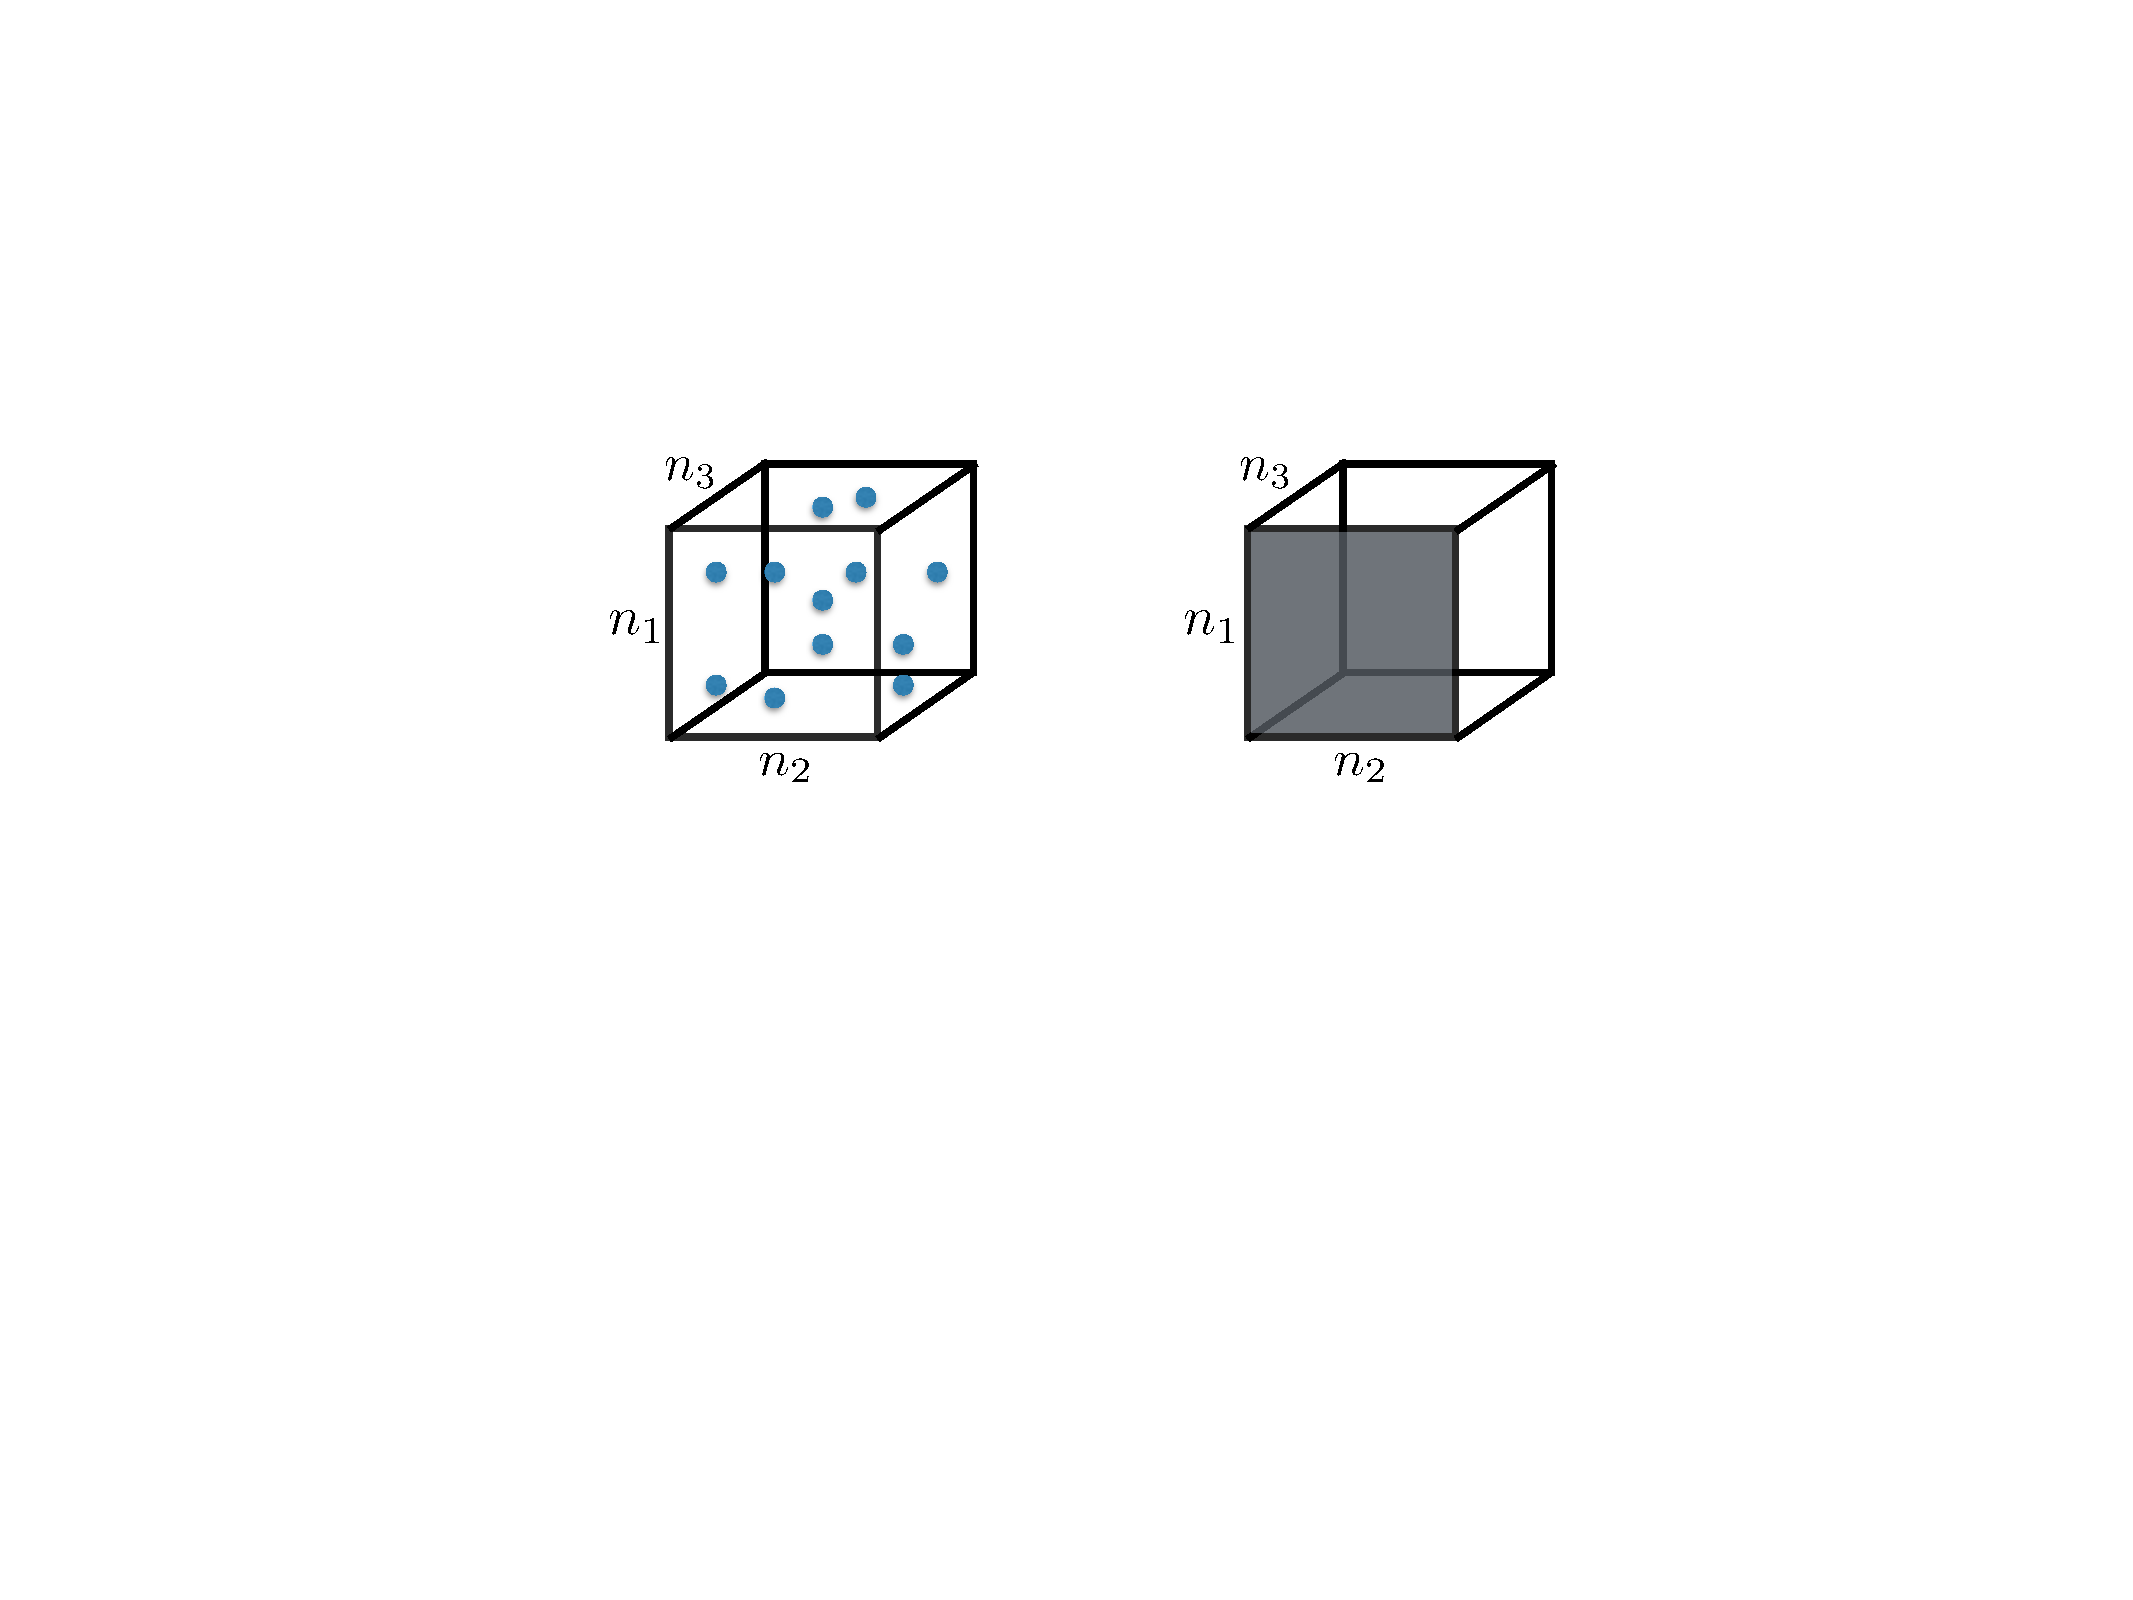
\includegraphics[width=0.6\linewidth]{thpropfigs/sparseanddense}
  \caption{A visualization of an order 3 ($d=3$) sparse and dense tensor (left and right, respectively.}
  \label{fig:sparseanddense}
\end{figure*}
An emerging area of research in computational science considers efficiently computing on data sets that are 
inherently multi-way-- that is, they can be represented by higher-order \emph{tensors}~\cite{Acar09futuredirections,Kolda:2009}. 
%
% Whereas matrix and block-matrix methods are widespread and well-understood in computational science, a current challenge is to develop \emph{tensor}-level thinking that deals with the unique challenges of tensor data sets~\cite{Acar09futuredirections}. 
%
% Tensor \emph{decompositions} are a leading method for compressing or finding structure within these 
% data sets, and increasing the computational scalability of these decompositions is an open research problem.
Tensor \emph{decompositions} are a powerful tool for the analysis of multi-way data, with many applications including including chemometrics~\cite{chemometrics}, quantum chemistry~\cite{quantumsurvey}, neuroscience~\cite{eegsurvey}, healthcare~\cite{rubik}, and deep learning~\cite{ttnn}. Tensor decompositions generally attempt to express an input tensor in a form that is lower-dimensional or of a more desirable structure. The resulting decomposition may be valuable for its interpretability (e.g., for factor analysis), or as a compressed format that alleviates the curse of dimensionality. Two of the most popular decompositions are visualized in~\cref{fig:decomps}, and the storage costs of the decompositions mentioned in this proposal are shown in~\cref{tab:storagecosts}, where the original tensor has dimension $n_k$ in mode $k$ and the decomposition has rank $r_k$ in mode $k$. Typically, $r_k << n_k$.

\begin{table}[h]
\centering\footnotesize
\begin{tabular}{l l}
\textbf{Representation} & \textbf{Storage Cost} \\ \hline
 \text{Original Tensor} &  $\prod_k n_k = \bigO{n^d}$ \\
 \text{CP} & $\sum_k r_kn_k = \bigO{nr}$ \\
 \text{Tucker} & $\sum_k r_kn_k + \prod_k r_k = \bigO{r^d}$  \\
 \text{Tensor Train} &  $n_1 r_1 + n_d r_d + \sum_{k=2}^{d-1}r_{k-1}r_kn_k = \bigO{nr^2}$
\end{tabular}
\caption{Storage costs of tensor decompositions in this proposal.}
\label{tab:storagecosts}
\end{table}
%
% It is tempting to think of tensor computations as inherently more costly than matrix computations.
% A key argument of this proposal however is that the multi-way structure of tensors surprisingly creates numerous avenues for increasing scalability that are not available in the realm of matrix computations.

As we can see from this table, a full representation of tensor data can scale arbitrarily large (exponential in its order, if each dimension is of a similar size). It is thus desirable to develop decomposition algorithms that scale in kind. We propose to utilize \emph{randomized} methods towards this end.
Recent developments in randomized numerical linear algebra utilize techniques such as random projection and 
sampling to perform common operations such as low-rank 
decomposition and least squares much faster than traditional methods, with the 
drawback that error bounds must often be restated in probabilistic terms. A central motivation in this proposal is the belief that
the dimensionality of tensors lends itself \emph{particularly} well to these randomized methods. 

Towards this goal we propose to develop efficient, high-performance implementations of randomized algorithms for leading tensor decompositions. We demonstrate in our prior work that the \textsc{Candecomp/Parafac} (CP) decomposition can be performed with randomized least squares, and that the tensor structure actually produces favorable conditions for the algorithm-- in fact, the randomized algorithm can extract more robust features than the leading deterministic algorithm at much lower cost~(\cref{sec:cp}). 

In addition we target scaling up the Tucker decomposition in distributed memory using methods drawn from the randomized SVD~(\cref{sec:tucker}), and propose that the tensor structure also suits both this method and another computation, the Tensor Train decomposition~(\cref{sec:tt}). 
%
\begin{figure}[ht]
  \centering 
  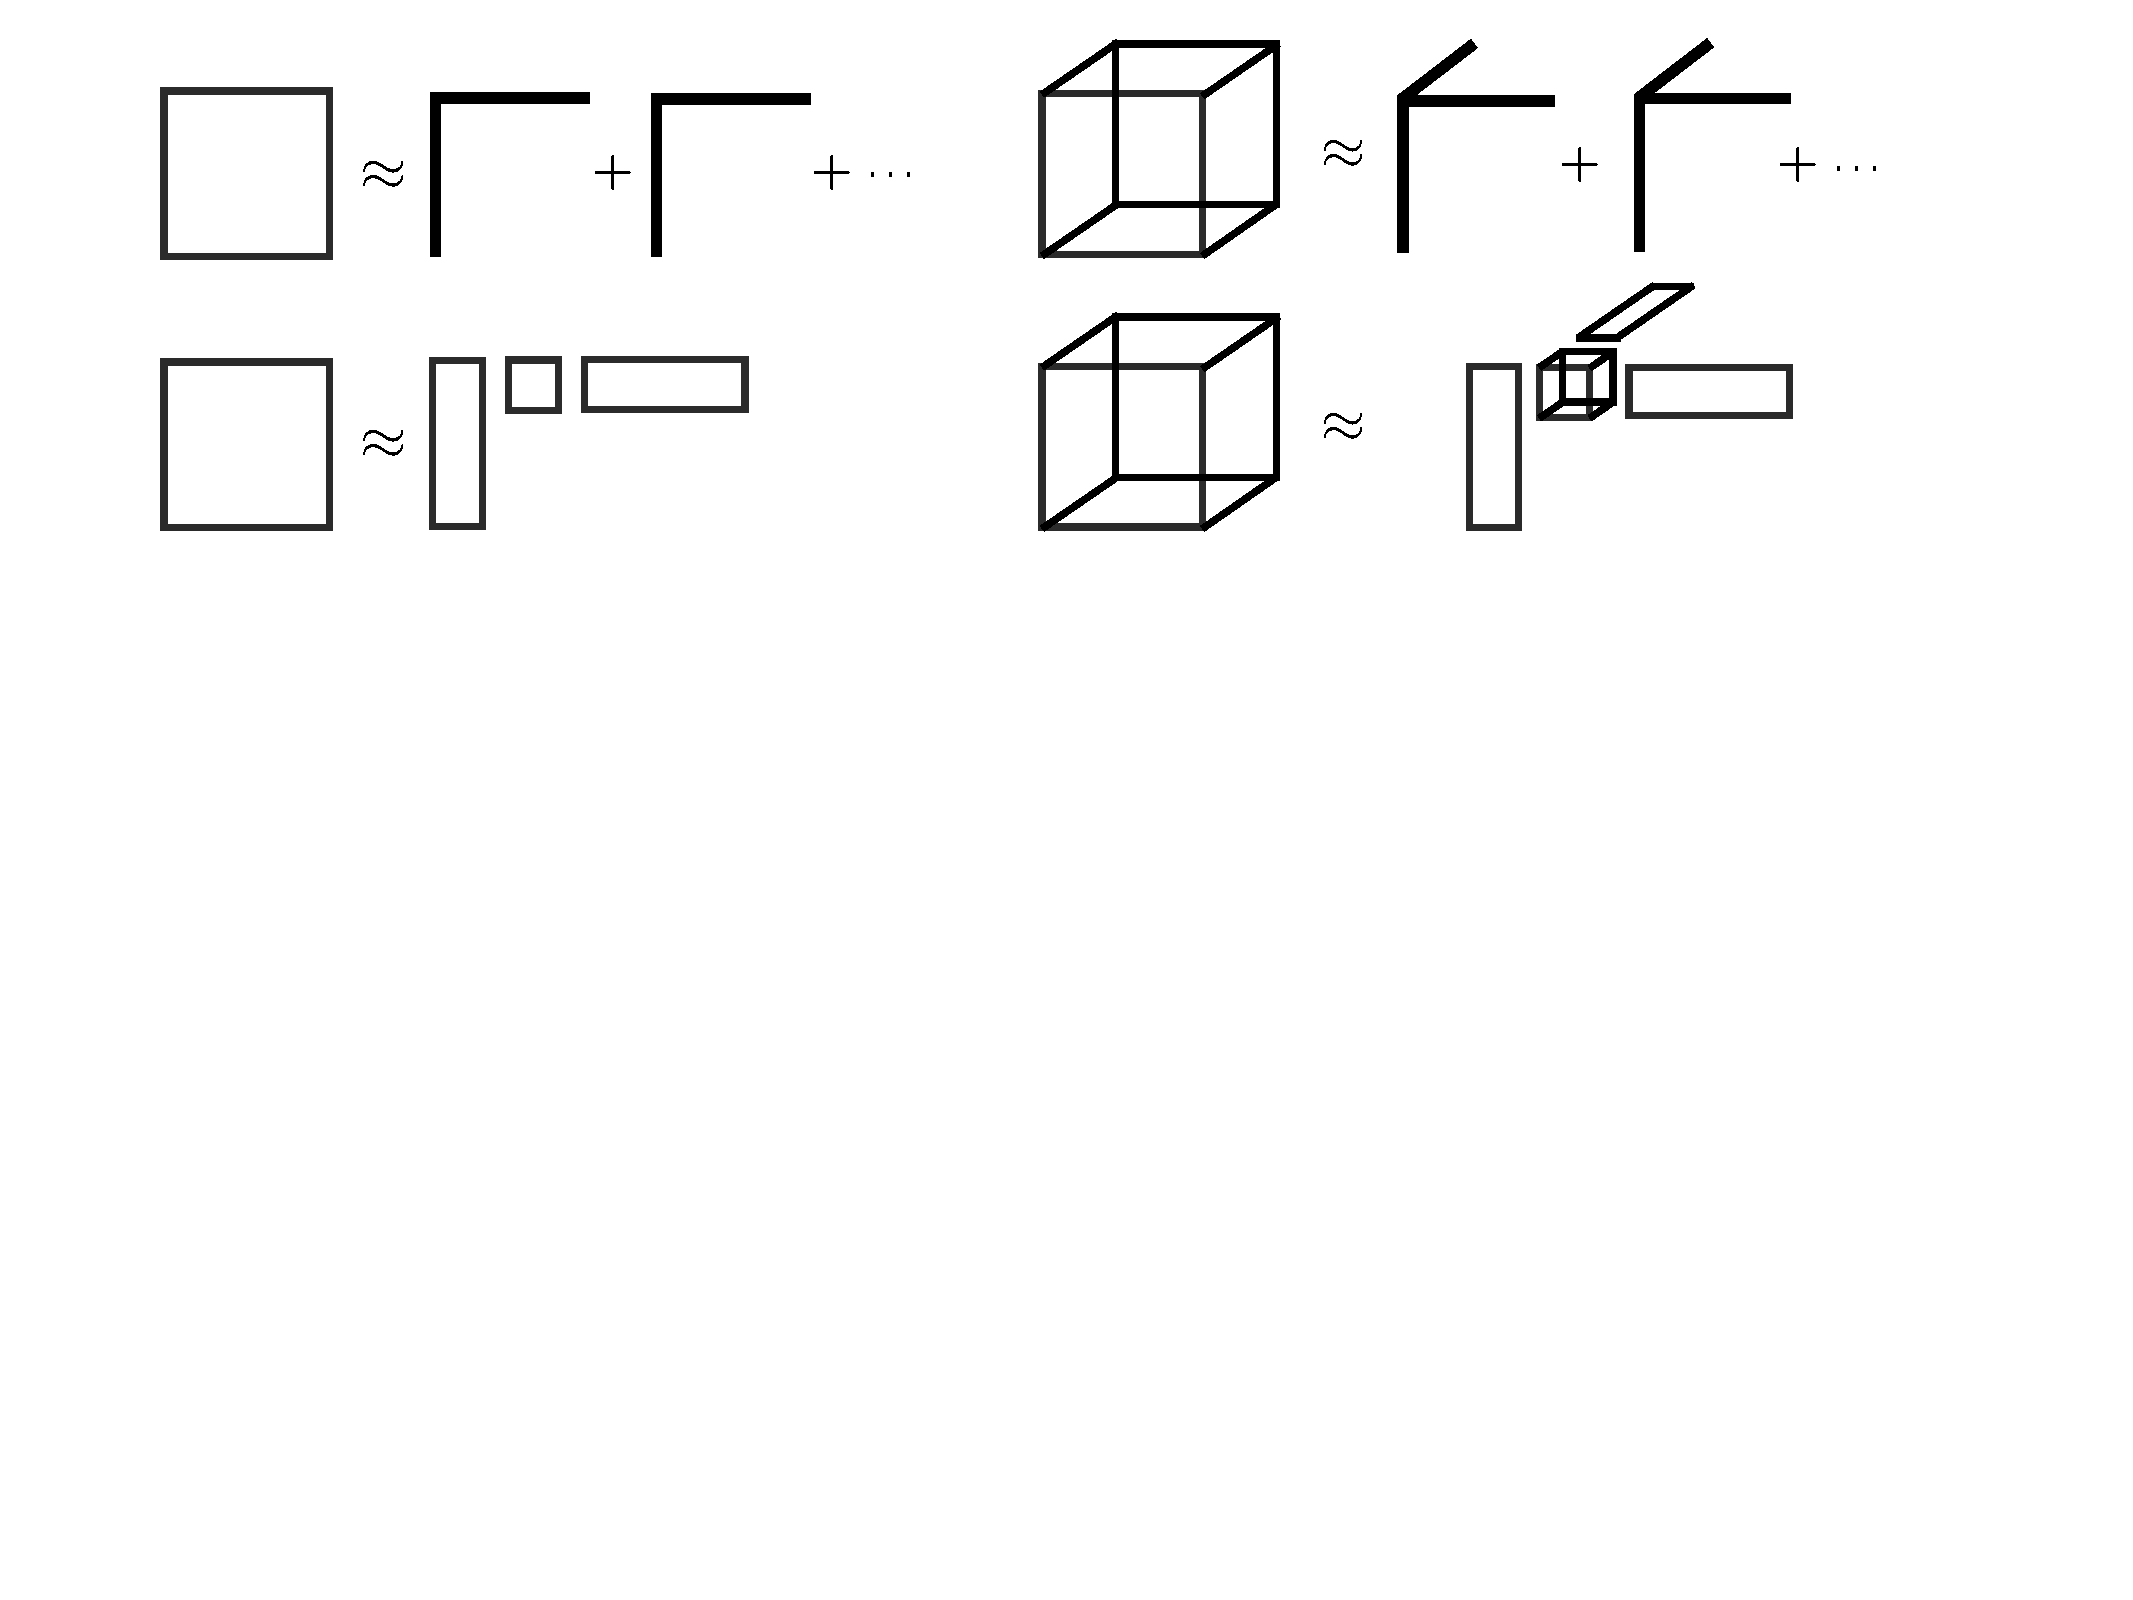
\includegraphics[width=\linewidth]{thpropfigs/decomps}
  \caption{Left: A low-rank matrix decomposition, visualized as a sum of rank-one matrices (top) or as a product of smaller matrices (bottom). Right: The CP decomposition, which is a sum of rank-one tensors (top), and the Tucker decomposition, which is a product of a smaller tensor with $d$ factor matrices in each mode (bottom).}
  \label{fig:decomps}
\end{figure}
%
\begin{figure}[ht]
  \centering 
  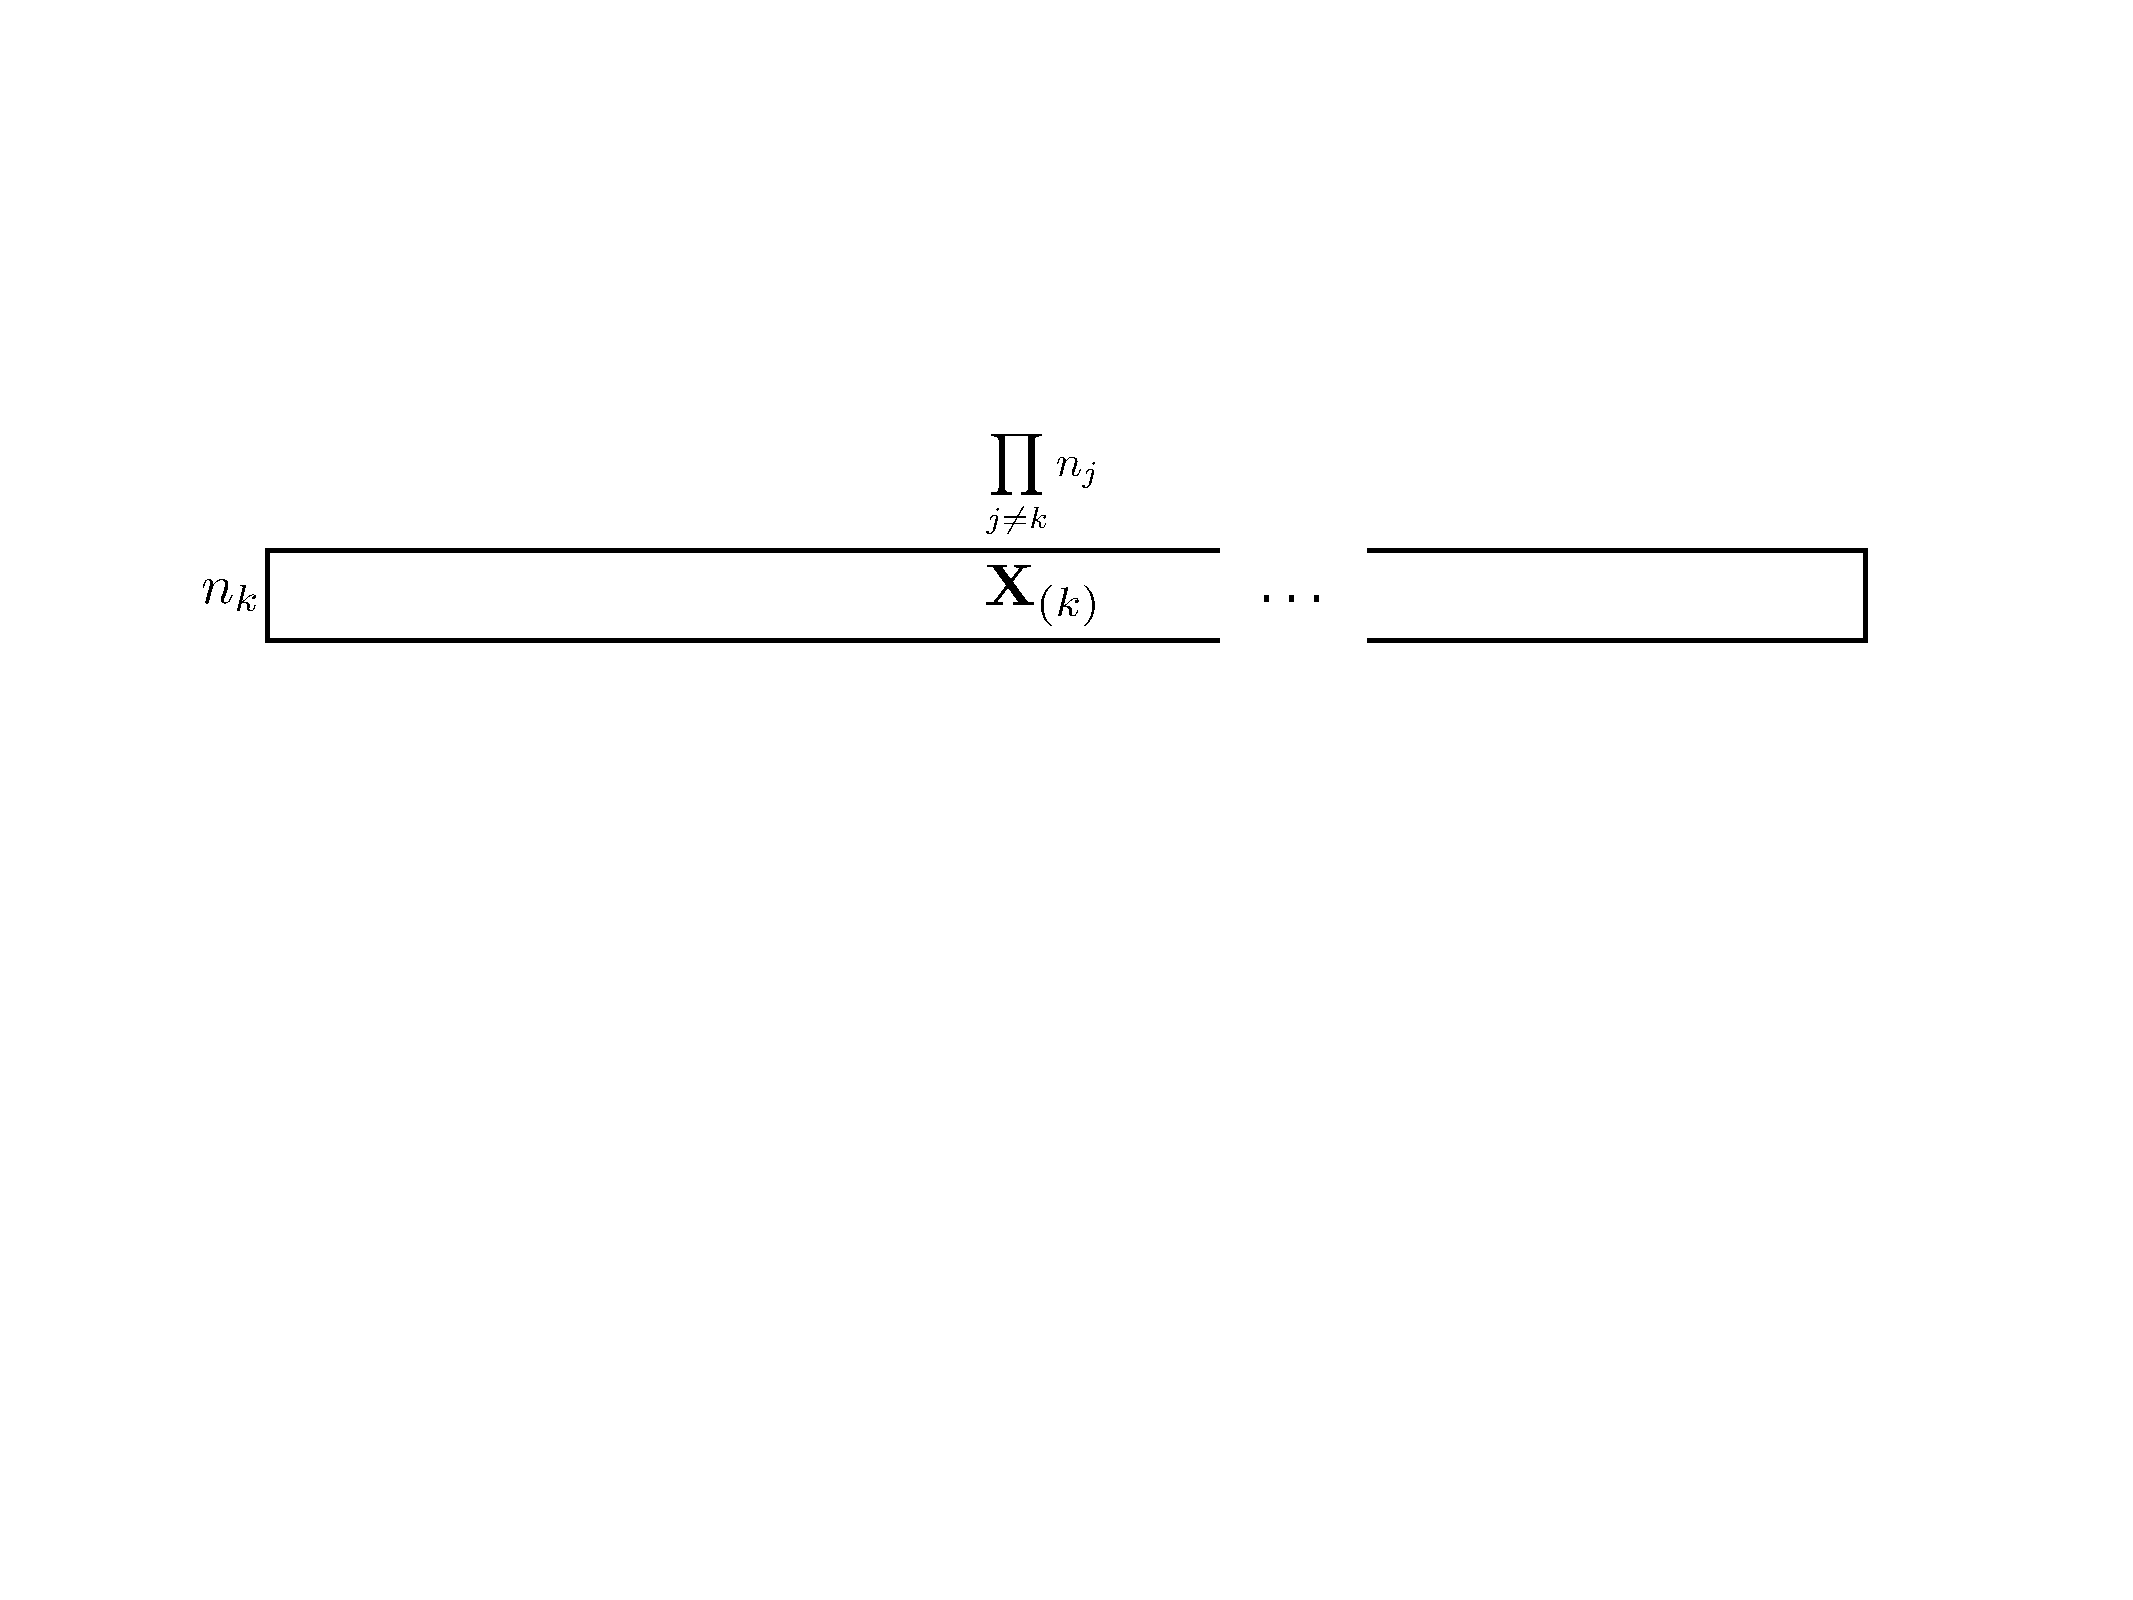
\includegraphics[width=0.85\linewidth]{thpropfigs/overdetermine}
  \caption{Intermediate computations in tensor decompositions often involve matrices where one dimension is much larger than the other. This is one example of a feature that is easily exploitable by randomized methods.}
  \label{fig:overdetermine}
\end{figure}
%
\subsection{Proposal}
We propose a line of research to apply sketching techniques to tensor decompositions, and to leverage them in such a way that allows for high-performance algorithms that outperform the state of the art. A key aspect within each decomposition is to show how sketching algorithms can leverage the specific higher-order structure of tensors.
\begin{enumerate}
\item \textsc{Candecomp/Parafac} (CP) Decomposition
\begin{itemize}
	\item The leading method for computing the CP decomposition is CP-ALS, which performs iterative least-squares updates in each mode.
	\item In completed work~\cite{caseyb}, we use methods drawn from \emph{randomized least squares} and apply them to this core computation.
	\item We show that the intermediate tensor structure produces conditions favorable for sketching due to both the dimensionality and `mixing' incurred by the Khatri Rao product.
	\item We introduce a new termination condition for the CP decomposition that uses sampled entries from the original tensor, and probabilistically bound the quality of this condition using the Chernoff-Hoeffding inequality. 
	\item We demonstrate scalability on real and synthetic data sets.
	\item We demonstrate the surprising result that this method often works \emph{better} than CP-ALS, returning good solutions more robustly.
	\item Deliverable: this method is published~\cite{caseyb} and released as part of MATLAB Tensor Toolbox~\cite{TTB_Software}\footnote{\url{http://gitlab.com/tensors/tensor_toolbox}}.
\end{itemize}
\item Tucker Decomposition / HOSVD
\begin{itemize}
	\item The leading method for computing the Tucker decomposition is the HOSVD, which performs mode-wise SVDs followed by tensor contractions.
	\item We propose to apply ideas from the Randomized SVD to the HOSVD in distributed memory.
	\item We propose that the tensor structure makes random projection highly efficient because it can be expressed as a series of small tensor contractions without intermediate communication. 
	\item We propose that the tensor structure uniquely allows for high-quality output because the efficiency of projections allows for significant \emph{oversampling} in very little time.
	\item We propose to demonstrate scalability on massive real and synthetic data sets on up to 1000 nodes.
	\item Deliverable: this method will be submitted for publication and included as part of TuckerMPI\footnote{\url{http://tensors.gitlab.io/TuckerMPI/}}.
\end{itemize}
\item Tensor Train Decomposition
\begin{itemize}
	\item The tensor train decomposition is a leading low-rank representation for very high-order tensors.
	\item We propose exploring how the structure of the tensor train computation can be exploited by randomized methods in a way comparable to the previous two methods (CP/Tucker).
	\item We propose demonstration of scalability on massive real and synthetic data sets.
	\item We propose developing a practical framework for the tensor train and quantized tensor train that allows for randomization. 
\end{itemize}
\end{enumerate}